\section{Planificación}
En esta parte se describe toda la planificación llevada a cabo durante el desarrollo de este proyecto, detallando las diferentes reuniones e iteraciones realizadas. En la figura \ref{fig:gantt} se puede apreciar el diagrama de \textbf{\textit{Gantt}} donde se indican las diferentes fases del proyecto.
\begin{figure}[H]
    \centering
    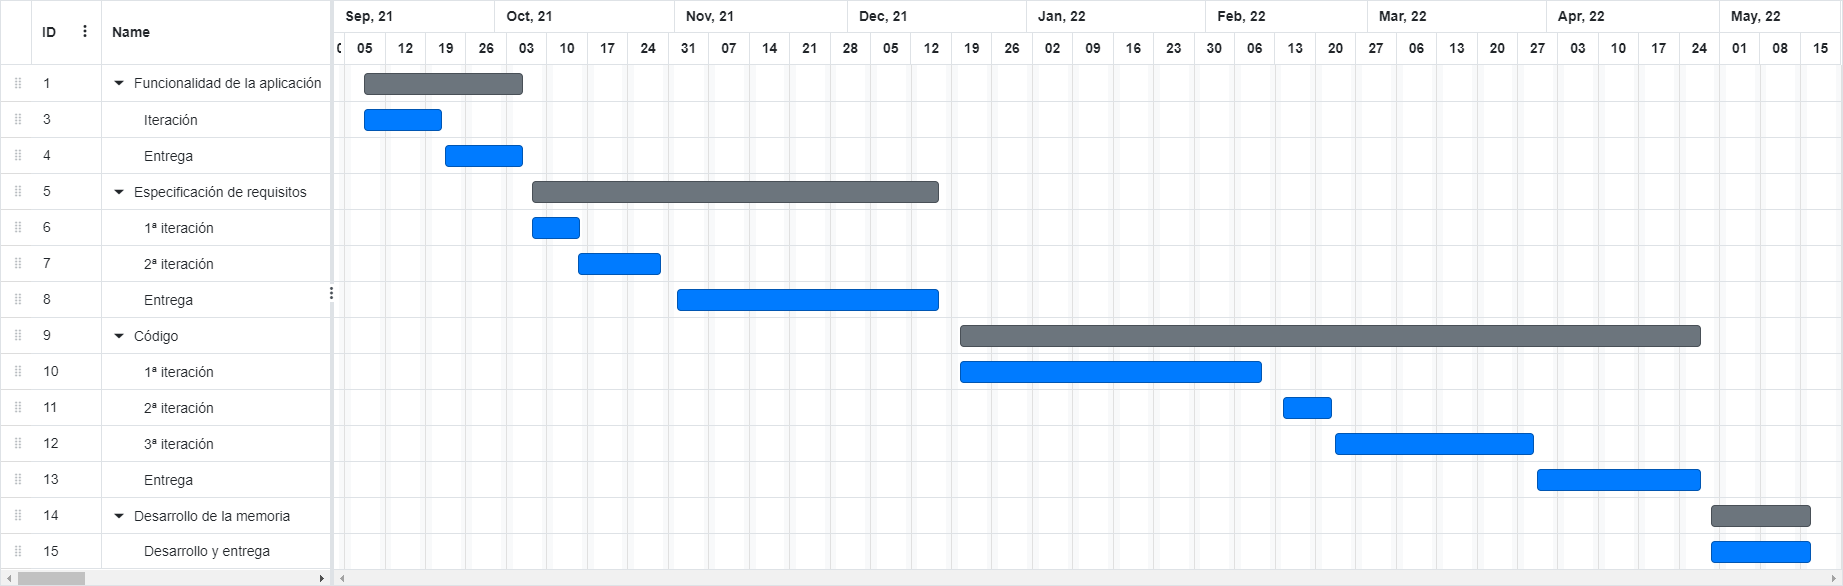
\includegraphics[width=\textwidth]{Images/gantt.png}
    \caption{Diagrama de Gantt de la planificación del proyecto}
    \label{fig:gantt}
\end{figure}

Durante la primera fase se establecieron las principales funcionalidades de la aplicación. Una vez terminada dicha fase, se especificaron los requisitos así como los actores y módulos que componen la aplicación. Para ello se realizaron dos iteraciones con el fin de establecer los requisitos finales.

Posteriormente, se establecieron tres iteraciones de código, en cada una de ellas se desarrollaron los distintos módulos previamente establecidos (login, dieta , dieta actual). Tras realizar las iteraciones de código, se realizaron diferentes pruebas de caja blanca sobre los distintos casos de uso. En la última fase se desarrolló la memoria que complementa al código.

Para poder llevar a cabo las diferentes fases mencionadas anteriormente, el equipo realizó reuniones cada sábado, con el fin de establecer la funcionalidad que se iba a desarrollar durante la semana. A su vez las reuniones ayudaron a conocer que habían realizado los integrantes durante la semana anterior, así como intentar resolver de manera conjunta los problemas que iban surgiendo.